\documentclass[11pt]{article}

\usepackage[letterpaper,margin=1in]{geometry}
\usepackage[T1]{fontenc}
\usepackage{lmodern}
\usepackage{microtype}
\usepackage{amsmath}
\usepackage{booktabs}
\usepackage{tabularx}
\usepackage{longtable}
\usepackage{array}
\usepackage{makecell}
\usepackage{adjustbox}
\usepackage{graphicx}
\usepackage{xcolor}
\usepackage{tikz}
\usepackage{float}
\usepackage{pdflscape}
\usepackage{caption}
\usepackage{subcaption}
\usepackage{enumitem}
\usepackage{natbib}
\usepackage{hyperref}

\usetikzlibrary{arrows.meta,calc,positioning,shapes.geometric,shapes.multipart}

\graphicspath{{paper/figures/}{figures/}}

\hypersetup{
  colorlinks=true,
  linkcolor=black,
  citecolor=black,
  urlcolor=black,
  pdfauthor={},
  pdftitle={Evaluating DRL Portfolio Claims under Explicit Cross-Asset Frictions}
}

\setlength{\parindent}{0pt}
\setlength{\parskip}{0.65em}
\setlist[itemize]{leftmargin=1.4em}
\setlist[enumerate]{leftmargin=1.6em}
\captionsetup{font=small,labelfont=bf}
\renewcommand{\arraystretch}{1.18}
\emergencystretch=2em
\Urlmuskip=0mu plus 1mu\relax

\newcolumntype{Y}{>{\raggedright\arraybackslash}X}
\newcolumntype{L}[1]{>{\raggedright\arraybackslash}p{#1}}
\newcolumntype{C}[1]{>{\centering\arraybackslash}p{#1}}
\newcommand{\cashzero}{Zero-CASH}
\newcommand{\cashbil}{BIL-CASH}
% Generated by scripts/build_paper_seed_aggregated_comparison.py; do not edit.
\newcommand{\AlignedWeeks}{228}
\newcommand{\AlignedStartDate}{2022-01-07}
\newcommand{\AlignedEndDate}{2026-05-15}
\newcommand{\ZeroBestTDThreeMandateRank}{4}
\newcommand{\BilBestTDThreeMandateRank}{7}
\newcommand{\ZeroBestTDThreeSharpeRank}{10}
\newcommand{\BilBestTDThreeSharpeRank}{10}
\newcommand{\ZeroTDThreeSharpe}{0.7327}
\newcommand{\BilTDThreeSharpe}{0.7549}
\newcommand{\ZeroBestTDThreeLabel}{V3 clean macro cap 0.70}
\newcommand{\BilBestTDThreeLabel}{V7 macro+GARCH cap 0.80}
\newcommand{\AggressiveFeasibleCount}{3}
\newcommand{\TDThreeFeasibleCount}{0}
\newcommand{\ZeroParetoTDThreeCount}{2}
\newcommand{\BilParetoTDThreeCount}{1}
\newcommand{\ZeroBootstrapMeanDelta}{0.1559}
\newcommand{\ZeroBootstrapLower}{-0.6011}
\newcommand{\ZeroBootstrapUpper}{0.9767}
\newcommand{\ZeroBootstrapProbability}{0.629}
\newcommand{\ZeroWrcPValue}{0.7136}
\newcommand{\BilBootstrapMeanDelta}{0.1170}
\newcommand{\BilBootstrapLower}{-0.7172}
\newcommand{\BilBootstrapUpper}{0.9963}
\newcommand{\BilBootstrapProbability}{0.588}
\newcommand{\BilWrcPValue}{0.6767}

\definecolor{stackborder}{RGB}{70,78,88}
\definecolor{stackfill}{RGB}{246,247,248}
\definecolor{stackdark}{RGB}{225,229,234}

\title{\textbf{Evaluating DRL Portfolio Claims under Explicit Cross-Asset Frictions}\\
\large A TD3 Case Study with Costs, Cash, Benchmark Diagnostics, and Statistical Validation}
\author{}
\date{}

\begin{document}

\maketitle

\begin{abstract}
Financial deep reinforcement learning (DRL) portfolio results are difficult to interpret when weak benchmarks, simplified trading frictions, ambiguous cash treatment, and candidate search are compressed into a single backtest ranking. This paper proposes a falsification-oriented evaluation framework that separates ranking competitiveness, statistical credibility, and practical feasibility, using TD3 as a case-study learner rather than as an algorithmic contribution. The empirical test bed contains SPY, TLT, GLD, BTC-USD, and CASH under weekly long-only allocation, asset-specific transaction costs, explicit \cashzero{} and \cashbil{} protocols, deterministic benchmarks, and four walk-forward folds. All combined-ranking strategies are evaluated on the same \AlignedWeeks{} out-of-sample Fridays. TD3 metrics are computed on each complete seed history before taking their mean across ten seeds; deterministic benchmarks retain one aligned path. BuyHold GLD leads both combined rankings. The best TD3 by mandate-aware score is \ZeroBestTDThreeLabel{} under \cashzero{}, at ranks \ZeroBestTDThreeMandateRank{} and \ZeroBestTDThreeSharpeRank{} by mandate-aware score and canonical Sharpe; under \cashbil{}, \BilBestTDThreeLabel{} ranks \BilBestTDThreeMandateRank{} and \BilBestTDThreeSharpeRank{}, respectively. Pairwise mean-path bootstrap ranges cross zero, and White Reality Check does not support superiority for the retained five-candidate sets. No seed-aggregated TD3 passes a tested hard mandate profile, although three deterministic benchmarks pass the aggressive profile. The contribution is therefore an evaluation framework for delimiting claims, not a new TD3 variant or deployable alpha result. Generalization is limited by a compact mainly U.S. test bed, one historical market path, training-seed dispersion, and simplified execution modeling.
\end{abstract}

\section{Introduction}

Financial deep reinforcement learning (DRL) has become an appealing tool for portfolio allocation because it can learn dynamic allocation rules without imposing a closed-form return model. In continuous-action settings, algorithms such as TD3 can map market states into portfolio weights, adapt allocations over time, and internalize transaction costs through the environment. This makes DRL attractive for cross-asset allocation problems where the relevant decision is not a single buy-or-sell signal, but a sequence of portfolio weights.

The central challenge, however, is not producing a high-ranking backtest. It is determining whether that ranking survives a disciplined financial evaluation. In financial applications, apparent outperformance can be created or amplified by weak benchmarks, simplified trading costs, unclear cash treatment, candidate-search bias, unstable concentration, limited robustness analysis, or the absence of statistical controls for data snooping. A strategy may rank well in a backtest and still fail to establish a reliable economic advantage once these layers are imposed.

The empirical setting is a compact and interpretable wealth-allocation universe composed of five economic sleeves: equity growth, interest-rate duration, real safe-haven exposure, digital alternative risk, and defensive liquidity. These sleeves are proxied by SPY, TLT, GLD, BTC-USD, and CASH. The universe is deliberately narrow. It is not intended to approximate the full global market portfolio. It is designed as a controlled test bed where allocation behavior can be interpreted as rotation across distinct macro-financial exposures.

The central research question is:

\begin{quote}
\emph{Can a falsification-oriented evaluation framework distinguish ranking competitiveness, statistical credibility, and practical feasibility in TD3-based cross-asset portfolio allocation?}
\end{quote}

This paper addresses that question using TD3 as a continuous-control empirical test case. TD3 is well suited for portfolio-weight decisions, but the focus of the paper is the evaluation protocol surrounding the model: how benchmark comparability is audited, how cash is treated, how costs are imposed, how candidate search is controlled, and how ranking results are separated from statistical and practical claims.

The paper answers the research question through a falsification-oriented evaluation protocol. TD3 candidates are trained and evaluated in a weekly long-only portfolio environment with asset-specific costs and two explicit cash protocols: \cashzero{} and \cashbil{}. Deterministic benchmarks use the same asset universe, cost schedule, and cash assumption. The comparison layer intersects every strategy with the exact \AlignedWeeks{}-date TD3 out-of-sample index before recomputing metrics, scores, mandates, and Pareto frontiers. The subsequent bootstrap and White Reality Check address sampling uncertainty and retained-set search. Additional layers examine regime dependence, execution-spread sensitivity, and training-budget diagnostics.

The evidence leads to a deliberately cautious interpretation. The highest-ranked TD3 changes from V3 under \cashzero{} to V7 under \cashbil{}, but neither learning candidate leads its combined universe or reaches the upper canonical-Sharpe ranks. The statistical layer does not support dominance over Trend SPY/CASH. Cash assumptions therefore affect TD3 selection, while hard filters admit only three benchmarks under the aggressive profile. The main result is not that the case study wins or fails, but that explicit evaluation layers expose the boundary of each claim.

The paper makes four contributions. First, it specifies an evaluation hierarchy for DRL-based cross-asset allocation with explicit cash assumptions and asset-specific costs. Second, it provides an exact-date comparison layer with source hashes, aligned histories, and executable checks that prevent horizon mismatch. Third, it separates ranking from pairwise uncertainty and retained-set evidence through block-bootstrap ranges and White Reality Check. Fourth, it adds practical diagnostic layers covering mandate feasibility, Pareto tradeoffs, regime dependence, execution-spread stress, and training-budget sensitivity.

The contribution is a disciplined evaluation framework for interpreting DRL portfolio evidence. Under this framework, competitiveness, statistical credibility, and practical feasibility are treated as separate claims rather than collapsed into a single backtest ranking.

\subsection{Empirical Propositions}

Five compact propositions organize the tests. \textbf{P1} asks whether at least one TD3 candidate remains ranking-competitive against deterministic benchmarks under common financial and date assumptions. \textbf{P2} asks whether any observed ranking advantage survives pairwise sampling uncertainty and candidate-set data-snooping control. \textbf{P3} asks whether cash treatment and additional execution frictions change selection or economic interpretation. \textbf{P4} asks whether a favorable ranking also satisfies hard practical constraints. \textbf{P5} asks whether regime and training-budget diagnostics narrow the apparent robustness of the selected policies. These propositions define an evidentiary sequence; none treats a first-place diagnostic rank as sufficient evidence of statistical superiority or deployability.

\section{Related Literature and Research Gap}

\subsection{DRL Portfolio Allocation and Evaluation Fragility}

Portfolio allocation is a natural application of reinforcement learning because portfolio weights are sequential decisions and realized performance depends on the interaction between returns, costs, and previous allocations. Earlier portfolio theory formalized mean-variance tradeoffs, performance evaluation, and dynamic portfolio choice \citep{markowitz1952,sharpe1966,merton1969,merton1971}. DRL extends this setting by learning allocation rules from historical state variables rather than specifying a parametric return model.

Twin Delayed Deep Deterministic Policy Gradient (TD3) is an established continuous-control actor-critic algorithm built on deterministic policy gradients, twin critics, delayed actor updates, target networks, and target policy smoothing \citep{silver2014,lillicrap2015,fujimoto2018}. Its continuous-action structure is suitable for portfolio-weight decisions, which makes it a useful empirical case study for evaluating DRL portfolio claims under explicit financial assumptions.

Prior work has already studied recurrent reinforcement learning for trading, model-free DRL portfolio management, FinRL-style trading frameworks, risk-aware portfolio rewards, correlation-aware DRL portfolio selection, and TD3 portfolio-selection models \citep{moody2001,jiang2017,almahdi2017,liu2020finrl,zhao2023correlation,jiang2024td3,jiang2025multiperiod}. The question here is narrower and more severe: which apparent DRL portfolio advantages remain defensible when explicit evaluation layers are imposed together.

\subsection{Multi-Asset and Crypto/Gold Portfolio Allocation}

The empirical universe is designed around a compact wealth-allocation problem under macro-financial uncertainty. At each rebalancing date, the allocation decision is not simply whether to hold more or less risky assets, but how to rotate capital across economically distinct sources of portfolio risk: equity growth exposure, interest-rate duration, defensive liquidity, real safe-haven exposure, and digital alternative risk. SPY, TLT, CASH/BIL, GLD, and BTC-USD are therefore used as liquid proxies for these five allocation sleeves. The universe is deliberately compact rather than exhaustive, so allocation behavior can be interpreted through economically meaningful risk categories rather than through a large opaque asset set.

This compact design is consistent with work that studies Bitcoin inside traditional stock-bond or multi-asset portfolio settings, including out-of-sample allocation, transaction costs, liquidity, and institutional portfolio-construction perspectives \citep{platanakis2020bitcoin,hubrich2023bitcoin,petukhina2021digitalassets}.

Gold and Bitcoin have both been studied in portfolio, diversification, hedge, and safe-haven contexts, but the literature does not support treating Bitcoin as a simple substitute for gold \citep{bouri2017bitcoinhedge,henriques2018bitcoinGold,guesmi2019bitcoinDiversification,klein2018bitcoin}. They should not be treated as equivalent. Gold is a real safe-haven and hard-asset proxy with a long institutional history, not a broad commodity basket. Bitcoin is a speculative digital alternative with high volatility, adoption risk, and idiosyncratic market structure, not a replacement for gold and not the full crypto ecosystem. This paper includes both to test whether the learning candidate can allocate across distinct risk sleeves, not because Bitcoin is assumed to be digital gold.

\subsection{Transaction Costs, Constraints, and Cash in Portfolio Evaluation}

Transaction costs and constraints are not implementation details in portfolio evaluation. A dynamic strategy with high turnover can look attractive before costs and fragile afterward. Similarly, a strategy forced to remain invested in risky assets has a different opportunity set from a strategy allowed to allocate defensively. Prior DRL portfolio work has incorporated transaction costs or risk-aware objectives, and machine-learning portfolio construction has also emphasized diversification and concentration control \citep{moody2001,almahdi2017,chen2022,jiang2024td3}.

In many real-world wealth-management and institutional allocation settings, cash or near-cash instruments are not merely residual balances. They represent liquidity, optionality, operational flexibility, and defensive risk control. Treating cash explicitly therefore changes the allocation problem rather than only adding another asset label.

This paper makes cash explicit. The \cashzero{} protocol treats cash as a synthetic zero-return defensive sleeve. The \cashbil{} protocol replaces that assumption with a short-term Treasury ETF proxy and assigns a nonzero transaction cost. This design tests whether the cash assumption changes model selection. It also prevents the paper from hiding the opportunity cost of defensive allocation.

\subsection{Statistical Validation and Data-Snooping Controls}

Financial model selection is vulnerable to data snooping. When many candidate policies are trained and evaluated, the best observed strategy may look strong because of the search process rather than because of a reliable economic edge. White's Reality Check directly addresses data-snooping risk, while Deflated Sharpe and related backtest-overfitting work motivate caution when interpreting searched strategy performance \citep{white2000,bailey2014,lopezdeprado2020mlam}.

This paper uses pairwise bootstrap risk-adjusted-return ranges and White Reality Check p-values as statistical guardrails. These tests do not replace economic interpretation, but they prevent ranking results from being overstated as statistical dominance.

\subsection{Research Gap and Literature Positioning}

The research gap is not any single ingredient in isolation---TD3, Bitcoin, transaction costs, cash, or statistical testing. Each appears in adjacent literatures. The gap lies in how these ingredients are combined and interpreted: few DRL portfolio studies jointly audit benchmark comparability, explicit cash assumptions, asset-specific frictions, statistical validation, and practical robustness layers before translating performance into claims.

\begin{table}[H]
\centering
\caption{Research gap and literature positioning.}
\label{tab:research-gap}
\footnotesize
\setlength{\tabcolsep}{4.5pt}
\renewcommand{\arraystretch}{1.32}
\begin{adjustbox}{max width=\textwidth}
\begin{tabularx}{\textwidth}{@{}L{0.17\textwidth} L{0.25\textwidth} L{0.27\textwidth} Y@{}}
\toprule
Literature stream & What it typically does & Main limitation for the present question & What remains missing \\
\midrule
DRL portfolio allocation & Trains reinforcement-learning agents to map market states into allocation or trading decisions. & Often emphasizes model performance without fully isolating the evaluation assumptions that support the result. & A protocol that treats ranking, statistical credibility, and practical feasibility as separate claims. \\
TD3-based portfolio studies & Uses TD3 as a continuous-control allocator for portfolio weights or trading actions. & The algorithmic choice can be foregrounded more than the evidentiary discipline around the backtest. & A TD3 evaluation framed as a stress test of claims rather than as a claim of TD3 novelty. \\
Multi-asset allocation with Bitcoin and alternative assets & Studies diversification, hedge behavior, and allocation across conventional and alternative assets. & Including alternative assets does not by itself resolve benchmark matching, cash treatment, or model-selection bias. & An interpretable cross-asset test bed where alternative-risk exposure is evaluated under matched financial assumptions. \\
Portfolio studies with transaction costs and practical frictions & Adds trading costs, constraints, turnover analysis, or implementation frictions. & Frictions are often examined as isolated adjustments rather than as part of a unified validation stack. & Joint treatment of asset-specific costs, explicit cash protocols, execution-spread stress, and feasibility filters. \\
Robustness and statistical evaluation in quantitative finance & Uses bootstrap methods, data-snooping controls, and robustness checks to discipline performance claims. & These tools are not always integrated into DRL portfolio model selection and benchmark comparison. & A falsification-oriented pipeline linking searched TD3 candidates, aligned benchmarks, pairwise bootstrap ranges, White Reality Check, and practical robustness layers. \\
\bottomrule
\end{tabularx}
\end{adjustbox}
\end{table}

The contribution is therefore the integrated evaluation design. This paper asks whether apparent DRL portfolio advantages, instantiated through a TD3 case study, remain competitive, statistically credible, and practically feasible after benchmark diagnostics, asset-specific frictions, explicit cash assumptions, date-aligned statistical validation, and robustness layers are imposed together.

\section{Data and Asset Universe}

Table~\ref{tab:asset-universe} operationalizes the five-sleeve design introduced above. The objective is not to represent the full global market portfolio, but to preserve an interpretable cross-asset test bed in which allocation behavior can be traced to growth risk, duration risk, defensive liquidity, real safe-haven exposure, and digital alternative risk. Broader universes are therefore best treated as future validation rather than as a problem this paper claims to solve.

\begin{table}[htbp]
\centering
\caption{Asset universe and economic risk sleeves.}
\label{tab:asset-universe}
\small
\begin{tabularx}{\textwidth}{L{0.12\textwidth} L{0.19\textwidth} Y Y}
\toprule
Asset & Economic role & Interpretation & Limitation \\
\midrule
SPY & Equity / growth risk & Broad U.S. equity exposure and the main pro-cyclical growth sleeve. & U.S.-centric equity proxy; not a global equity portfolio. \\
TLT & Duration / interest-rate risk & Long-duration Treasury exposure used to represent interest-rate duration risk. & Not generic fixed income and not risk-free; vulnerable to rate shocks. \\
GLD & Real safe-haven / hard-asset exposure & Gold exposure used as a real safe-haven and hard-asset sleeve. & Not cash and not a broad commodity basket. \\
BTC-USD & Digital alternative / speculative convexity & High-volatility digital alternative asset with asymmetric upside and idiosyncratic risk. & Not assumed to be digital gold; not the full crypto ecosystem; large drawdown and liquidity risk. \\
CASH & Defensive liquidity / optionality & Allows the policy to reduce risky exposure and preserve liquidity optionality. & Synthetic under \cashzero{}; BIL is only a proxy for investable cash. \\
\bottomrule
\end{tabularx}
\end{table}

The resulting universe is compact and deliberately incomplete. It excludes credit, real estate, broad commodities, international equities, taxes, custody costs, and investor-specific liabilities. These exclusions keep the empirical setting interpretable while making clear that the design is a controlled test bed, not a complete investable universe.

Adjusted-close prices are aligned to Friday observations and converted to simple weekly returns. The underlying return files span 9 January 2015 to 15 May 2026; usable candidate histories begin later when feature availability and the one-period information lag remove early rows. State variables available through (t-1) determine weights for (t), and the next weekly return is then realized. This timing convention, together with the expanding walk-forward splits reported in Appendix~\ref{app:protocol-detail}, reduces look-ahead risk without creating independent market histories.

The cash dimension is implemented through two protocols.

\begin{table}[htbp]
\centering
\caption{Cash protocols.}
\label{tab:cash-protocols}
\small
\begin{tabularx}{0.92\textwidth}{L{0.18\textwidth} L{0.22\textwidth} L{0.17\textwidth} Y}
\toprule
Protocol & Return assumption & Cost assumption & Interpretation \\
\midrule
\cashzero{} & 0 return & 0 bps & Synthetic defensive sleeve used to isolate allocation behavior. \\
\cashbil{} & BIL proxy return & 2 bps & Short-term Treasury ETF proxy used as cash-assumption robustness. \\
\bottomrule
\end{tabularx}
\end{table}

The two protocols are not interchangeable. They define different investable environments and therefore can produce different preferred TD3 specifications.

\section{Empirical Design and Learning Setup}

\subsection{Portfolio Environment}

At each weekly decision date, the agent selects long-only portfolio weights over SPY, TLT, GLD, BTC-USD, and CASH. Weights sum to one across all available sleeves, but risky-asset exposure can fall below one because CASH is part of the investable universe.

Portfolio performance is measured after transaction costs. Let \(w_{t,i}^{target}\) be the target weight in asset \(i\) at week \(t\), \(w_{t-1,i}^{target}\) the previously executed target weight, \(r_{t,i}\) the asset return, and \(c_i\) the asset-specific one-way cost rate. The final histories use target-to-prior-target turnover rather than post-return drifted weights. The gross portfolio return is:
\begin{equation}
R^{gross}_t = \sum_i w^{target}_{t,i} r_{t,i}.
\end{equation}

The transaction cost is:
\begin{equation}
C_t = \sum_i c_i \left|w^{target}_{t,i} - w^{target}_{t-1,i}\right|.
\end{equation}

The net financial return is:
\begin{equation}
R^{net}_t = R^{gross}_t - C_t.
\end{equation}

The corrected cost schedule is asset-specific: SPY, TLT, and GLD use 2 bps; BTC-USD uses 10 bps; CASH uses 0 bps under \cashzero{} and 2 bps under \cashbil{}. The schedule is a transparent modeling assumption informed by public broker and exchange fee schedules, including Interactive Brokers for ETF/equity trading and Binance for crypto trading fees \citep{interactivebrokers2026commissions,binance2026tradingfees}. It should not be interpreted as an exact account-specific execution-cost estimate.

\subsection{Case-Study Learning Agent}

The learning agent is TD3, a continuous-control actor-critic model. The actor maps state variables into portfolio weights. Twin critics reduce overestimation bias. The algorithm uses a replay buffer, target networks, target policy smoothing, delayed actor updates, and behavior-policy exploration during training. Evaluation is deterministic.

In this design, TD3 functions as the case-study learner. It is used because portfolio allocation is a continuous-action problem and because TD3 is a standard benchmark algorithm for deterministic continuous control.

\subsection{Feasible Action Handling}

Portfolio actions are projected consistently before execution and storage so that the policy, environment, replay buffer, and critic updates operate on feasible weights. This is a methodological safeguard. It is not framed as a separate algorithmic contribution.

\subsection{Reward}

The reward uses net financial return after transaction costs and a unit-weight current-drawdown penalty. With \(M_t=\max_{s\leq t}V_s\), current drawdown severity is \(DD_t=\max(0,1-V_t/M_t)\), and the final configuration uses:
\begin{equation}
reward_t = R^{net}_t - DD_t.
\end{equation}

Transaction costs therefore affect both realized performance and the training signal. The return and drawdown coefficients are one; direct turnover and concentration coefficients are zero, and mandate/cash penalties are disabled. Turnover and concentration are evaluated through costs, max-weight caps, diagnostics, mandate profiles, and Pareto analysis. The paper does not train on the final custom evaluation scores.

\subsection{Feature Families}

The experiment evaluates multiple TD3 feature families rather than one manually selected state representation. The objective is to test which independently trained state specification survives a common evaluation protocol; volatility-state variants use generalized autoregressive conditional heteroskedasticity (GARCH) information \citep{bollerslev1986}.

\begin{table}[htbp]
\centering
\caption{TD3 feature families.}
\label{tab:feature-families}
\small
\begin{tabularx}{\textwidth}{L{0.18\textwidth} Y Y}
\toprule
Candidate & Description & Role in experiment \\
\midrule
V2 reference & Broad reference financial state. & Baseline rich feature set for comparison. \\
V3 clean macro & Financial state plus clean real-time/as-of macro variables. & Tests whether audited macro information improves allocation. \\
V4 GARCH & Financial state plus fitted GARCH-style volatility features. & Tests volatility-forecast feature value. \\
V5 no-vol & Ablation excluding a volatility feature block. & Tests whether simpler non-volatility states remain competitive. \\
V6 financial & Parsimonious financial state with renamed score-like indicators. & Tests compact financial state representation. \\
V7 macro+GARCH & Clean no-DXY macro state plus GARCH features. & Tests whether GARCH improves the clean macro specification. \\
V8 EWMA/GARCH & Exponentially weighted moving average (EWMA)/GARCH volatility hybrid. & Tests alternative volatility-state construction. \\
\bottomrule
\end{tabularx}
\end{table}

Short candidate labels are used for readability; full feature-family identifiers are reported in the project outputs. The clean macro/as-of pipeline excludes the U.S. Dollar Index (DXY) because a full-window fresh true-vintage dollar proxy is not available without fallback, discontinuation, or current-vintage relabeling. CPI year-over-year is computed before weekly alignment. Heuristic probability-like V6 features are treated as scores rather than calibrated probabilities. Mechanical duplicate features are removed. Principal component analysis (PCA) was audited but is not used as the default state representation.

The registry in Table~\ref{tab:feature-families} records the broader candidate-design space. The final corrected 800-history grid per cash protocol is narrower and fully enumerated: V3, V4, V5, V7, and V8, crossed with four concentration settings (uncapped, 0.50, 0.70, and 0.80), ten seeds, and four folds. V2 and V6 remain reference designs in the broader registry but are not counted in that 800-history final grid. This distinction prevents the candidate registry from being confused with the final comparison sample.

\section{Falsification-Oriented Evaluation Protocol}

The learning setup above defines the case study. The methodological contribution lies in the evaluation stack imposed around it. The protocol makes its frictions and remaining comparability limits explicit rather than treating one ranking as sufficient evidence.

\subsection{Protocol System Overview}

\begin{figure}[H]
\centering
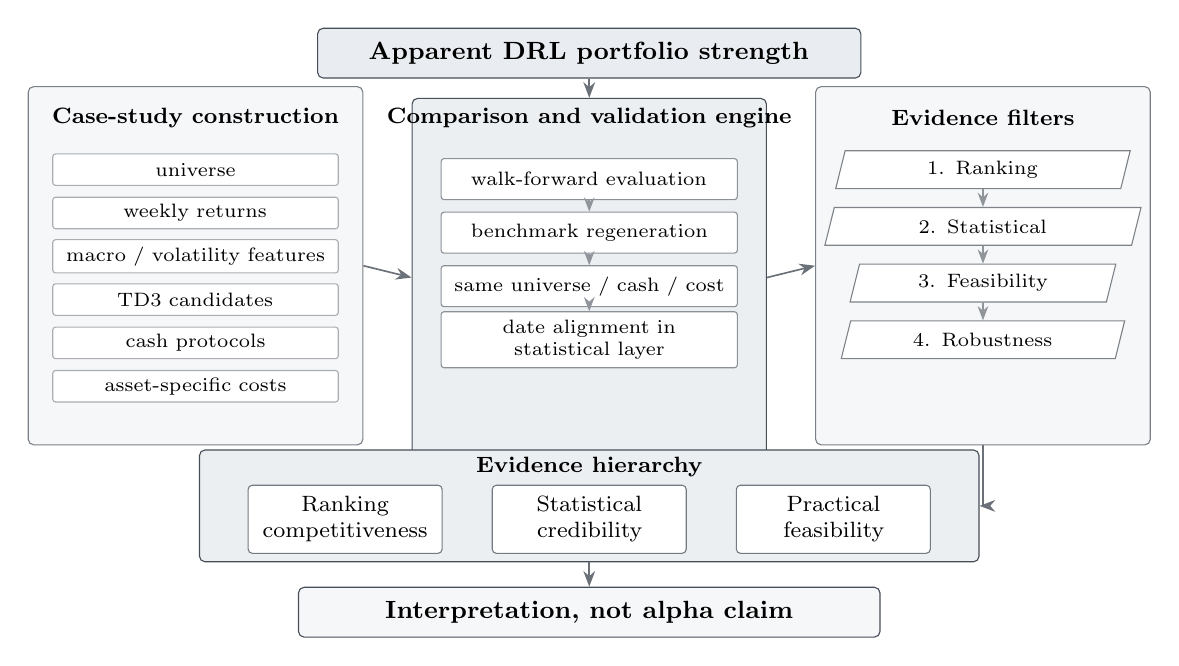
\begin{tikzpicture}[
  panel/.style={draw=stackborder!72, rounded corners=2pt, fill=stackfill, minimum width=4.25cm, minimum height=4.55cm},
  engine/.style={draw=stackborder, rounded corners=2pt, fill=stackdark!62, minimum width=4.50cm, minimum height=4.55cm},
  title/.style={font=\footnotesize\bfseries, align=center, text=black},
  item/.style={draw=stackborder!46, rounded corners=1pt, fill=white, align=center, text width=3.45cm, minimum height=0.40cm, inner sep=2.5pt, font=\scriptsize},
  core/.style={draw=stackborder!62, rounded corners=1pt, fill=white, align=center, text width=3.55cm, minimum height=0.52cm, inner sep=3pt, font=\scriptsize},
  gate/.style={trapezium, trapezium left angle=76, trapezium right angle=104, draw=stackborder!70, fill=white, align=center, text width=3.05cm, minimum height=0.48cm, inner sep=2.5pt, font=\scriptsize},
  output/.style={draw=stackborder, rounded corners=2pt, align=center, text width=0.72\textwidth, minimum height=0.62cm, inner sep=5pt, fill=stackdark!72, font=\small\bfseries},
  hierarchy/.style={draw=stackborder, rounded corners=2pt, fill=stackdark!62, minimum width=9.9cm, minimum height=1.42cm},
  claim/.style={draw=stackborder!75, rounded corners=1.5pt, align=center, text width=0.18\textwidth, minimum height=0.52cm, inner sep=4pt, fill=white, font=\footnotesize},
  arrow/.style={-{Stealth[length=2mm]}, semithick, stackborder!80},
  softarrow/.style={-{Stealth[length=1.8mm]}, semithick, stackborder!60}
]
\node[output, text width=0.54\textwidth, minimum height=0.52cm] (apparent) at (0,0) {Apparent DRL portfolio strength};

\node[panel] (constructbox) at (-5.00,-2.70) {};
\node[engine] (enginebox) at (0,-2.85) {};
\node[panel] (filterbox) at (5.00,-2.70) {};

\node[title] at (-5.00,-0.82) {Case-study construction};
\node[item] (c1) at (-5.00,-1.48) {universe};
\node[item] (c2) at (-5.00,-2.03) {weekly returns};
\node[item] (c3) at (-5.00,-2.58) {macro / volatility features};
\node[item] (c4) at (-5.00,-3.13) {TD3 candidates};
\node[item] (c5) at (-5.00,-3.68) {cash protocols};
\node[item] (c6) at (-5.00,-4.23) {asset-specific costs};

\node[title] at (0,-0.82) {Comparison and validation engine};
\node[core] (e1) at (0,-1.60) {walk-forward evaluation};
\node[core] (e2) at (0,-2.28) {benchmark regeneration};
\node[core] (e3) at (0,-2.96) {same universe / cash / cost};
\node[core] (e4) at (0,-3.64) {date alignment in statistical layer};
\draw[softarrow] (e1) -- (e2);
\draw[softarrow] (e2) -- (e3);
\draw[softarrow] (e3) -- (e4);

\node[title] at (5.00,-0.82) {Evidence filters};
\node[gate, text width=2.70cm] (f1) at (5.00,-1.48) {1. Ranking};
\node[gate, text width=2.55cm] (f2) at (5.00,-2.20) {2. Statistical};
\node[gate, text width=2.40cm] (f3) at (5.00,-2.92) {3. Feasibility};
\node[gate, text width=2.25cm] (f4) at (5.00,-3.64) {4. Robustness};
\draw[softarrow] (f1) -- (f2);
\draw[softarrow] (f2) -- (f3);
\draw[softarrow] (f3) -- (f4);

\node[hierarchy] (evidencebox) at (0,-5.75) {};
\node[title] (evidence) at (0,-5.25) {Evidence hierarchy};
\node[claim] (claimrank) at (-3.10,-5.92) {Ranking\\competitiveness};
\node[claim] (claimstat) at (0,-5.92) {Statistical\\credibility};
\node[claim] (claimpractical) at (3.10,-5.92) {Practical\\feasibility};
\node[output, fill=stackfill, text width=0.58\textwidth, minimum height=0.56cm] (interpret) at (0,-7.10) {Interpretation, not alpha claim};

\draw[arrow] (apparent.south) -- (enginebox.north);
\draw[arrow] (constructbox.east) -- (enginebox.west);
\draw[arrow] (enginebox.east) -- (filterbox.west);
\draw[arrow] (filterbox.south) |- (evidencebox.east);
\draw[arrow] (evidencebox.south) -- (interpret.north);
\end{tikzpicture}
\caption{Experimental protocol as an evidence system. Apparent DRL portfolio strength is challenged through benchmark diagnostics, date-aligned statistical validation, practical feasibility checks, and robustness layers. These layers are interpretation gates and do not feed back into training or retrospectively replace the candidates used at earlier layers.}
\label{fig:protocol-overview}
\end{figure}

Figure~\ref{fig:protocol-overview} summarizes the order of evidence used to interpret the DRL case-study performance without treating a high ranking as sufficient proof of superiority. The contribution lies in this evaluation hierarchy rather than in TD3 itself. Exact date matching now occurs before the combined ranking and is retained through the statistical and practical layers.

\subsection{Comparison and Validation Rules}

The fourteen deterministic benchmarks are generated from the same weekly return files under the same cash protocol, universe, and cost schedule. They cover buy-and-hold sleeves, equal-weight portfolios, 60/40 allocation, defensive risk-off, momentum, risk-adjusted momentum, rolling Markowitz, rolling minimum variance, inverse-volatility risk parity, and Trend SPY/CASH; Appendix~\ref{app:protocol-detail} gives the complete registry. Their causal full-history signals, weights, returns, and costs are preserved, but reported rows are selected by exact timestamp intersection with the TD3 out-of-sample index. Each TD3 seed concatenates its four disjoint test folds to the same \AlignedWeeks{} dates. Every nonlinear metric is computed on each complete seed history first; the primary TD3 row is the arithmetic mean of the ten resulting metric values, with dispersion retained separately. This estimates expected performance over a random training seed. The date-wise mean return path is retained only as a synthetic diagnostic: it is neither one selected policy nor an implemented ten-agent ensemble.

The pre-existing statistical layer uses the same \AlignedWeeks{} dates but a different object: fold/seed TD3 returns are averaged by date before resampling. Its pairwise bootstrap therefore describes the synthetic average-return path, not the distribution of a randomly trained single policy. It uses 1,000 replications and 12-week blocks and does not adjust for candidate selection. Its legacy source field called ``Sharpe'' is renamed here the \emph{CAGR-to-annualized-volatility ratio}; the combined ranking instead uses the canonical weekly arithmetic mean divided by sample standard deviation, annualized by $\sqrt{52}$. The two estimators are not numerically interchangeable. White Reality Check does not use either ratio: it applies 2,000 centered 8-week block-bootstrap replications to weekly candidate-minus-benchmark net-return differentials over five retained policies. It adjusts only for that retained universe, not all 20 feature-cap configurations, and its p-value is not pair-specific. Because even the mechanically diversified mean path fails to support superiority, the evidence cannot establish a stronger expected-seed claim; a hierarchical seed-and-time inference design remains future work.

\begin{table}[htbp]
\centering
\caption{Final corrected experimental protocol.}
\label{tab:protocol}
\small
\begin{tabularx}{0.92\textwidth}{L{0.34\textwidth} Y}
\toprule
Component & Design \\
\midrule
Frequency & Weekly \\
Asset universe & SPY, TLT, GLD, BTC-USD, CASH \\
Allocation & Long-only, fully invested across available sleeves \\
Return-file window & 9 January 2015--15 May 2026; usable rows depend on feature alignment \\
Walk-forward design & Four expanding-window folds; one-year validation blocks and tests for 2022, 2023, 2024, and 2025--15 May 2026 \\
Final corrected grid & Five feature families $\times$ four cap settings $\times$ ten seeds $\times$ four folds \\
Episodes & 60 \\
TD3 histories per cash assumption & 800 \\
Benchmarks per cash assumption & 14 \\
Cash assumptions & \cashzero{} and \cashbil{} \\
Costs & Asset-specific transaction costs \\
Statistical validation & 228 aligned weeks; pairwise bootstrap and five-candidate White Reality Check \\
Additional robustness & Regime analysis, mandate/Pareto feasibility, execution-spread stress, training-budget convergence \\
\bottomrule
\end{tabularx}
\end{table}

The 800 histories per cash assumption should not be interpreted as 800 independent market samples. They share the same historical period, folds, and asset universe. Their purpose is to assess candidate, cap, seed, and fold behavior under a systematic evaluation protocol.

Because the project contains several reporting layers, the word ``best'' changes meaning across sections. Table~\ref{tab:reporting-layers} defines the layers and prevents descriptive ranking results from being confused with statistical or practical feasibility claims.

\begin{table}[H]
\centering
\caption{Evidence layers and claim boundaries.}
\label{tab:reporting-layers}
\scriptsize
\setlength{\tabcolsep}{3.2pt}
\renewcommand{\arraystretch}{1.12}
\begin{tabularx}{\textwidth}{L{0.15\textwidth} L{0.19\textwidth} L{0.18\textwidth} Y Y}
\toprule
Layer & Question & Evidence & What it establishes & What it does not establish \\
\midrule
TD3 screening & Which specification and cap lead inside the searched TD3 set? & Within-TD3 metrics and diagnostic scores. & Internal candidate selection. & Benchmark superiority. \\
Combined diagnostic ranking & How do selected TD3 policies rank on common dates? & Standard and diagnostic metrics over the same 228 timestamps. & Exact-window descriptive competitiveness. & Statistical superiority or live performance. \\
Statistical validation & Is the apparent edge distinguishable from uncertainty and search? & Pairwise mean-path CAGR-to-volatility bootstrap and weekly-return-differential WRC. & The supported statistical claim. & Expected-seed inference, practical feasibility, or live performance. \\
Regime diagnostics & Is performance broad-based? & Regime-level metric leaders. & Historical state dependence. & All-weather robustness. \\
Mandate / Pareto & Do strategies satisfy constraints and tradeoffs? & Hard filters and aligned frontiers. & Feasibility under tested thresholds and conditional non-dominance. & Universal suitability. \\
Spread stress & Does less favorable execution alter results? & Post-training return and Sharpe degradation. & Sensitivity to the tested spreads. & A new selected policy or live execution quality. \\
Training budget & Does 60 episodes look obviously insufficient? & 30/60/100/150-episode comparison. & A diagnostic against obvious undertraining. & Global optimization or convergence. \\
\bottomrule
\end{tabularx}
\end{table}

\section{Evaluation Results: Ranking and Statistical Evidence}

\subsection{Which TD3 Candidate Leads the Internal Screening?}

The first result is evaluated within the searched learning-candidate universe. This layer asks which TD3 case-study variant and cap are strongest before deterministic benchmarks are introduced. It is useful for understanding policy behavior, but it is not evidence that the learning approach beats benchmarks.

Under \cashzero{}, V5 no-vol cap 0.50 is selected by the within-TD3 diagnostic layer, with mandate-aware score 0.601124 and robust score 0.696702. Under \cashbil{}, that layer selects V8 EWMA/GARCH cap 0.70, with mandate-aware score 0.660435 and robust score 0.749958.

Mandate-aware and robust scores are diagnostic selection summaries. Financial interpretation relies primarily on standard metrics and statistical validation.

\begin{table}[htbp]
\centering
\caption{Case-study candidate selection and standard metrics.}
\label{tab:td3-only}
\footnotesize
\setlength{\tabcolsep}{4.5pt}
\renewcommand{\arraystretch}{1.18}
\begin{tabularx}{\textwidth}{@{}L{0.13\textwidth} Y C{0.08\textwidth} C{0.10\textwidth} C{0.10\textwidth} C{0.10\textwidth} C{0.10\textwidth}@{}}
\toprule
Cash & Selected TD3 & Cap & \makecell{Ann.\\ret.} & \makecell{Ann.\\vol.} & Sharpe & \makecell{Max\\DD} \\
\midrule
\cashzero{} & V5 no-vol cap 0.50 & 0.50 & 0.0667 & 0.1156 & 0.5686 & -0.1206 \\
\cashbil{} & V8 EWMA/GARCH cap 0.70 & 0.70 & 0.0731 & 0.1060 & 1.0253 & -0.1066 \\
\addlinespace[0.45em]
\multicolumn{7}{@{}l}{\emph{Diagnostics and selection scores}} \\
\midrule
Cash & \multicolumn{2}{l}{Turnover} & \makecell{Eff.\\assets} & \makecell{Weekly\\cost} & \makecell{Mandate-\\aware} & Robust \\
\midrule
\cashzero{} & \multicolumn{2}{l}{0.4195} & 2.8093 & 0.000115 & 0.601124 & 0.696702 \\
\cashbil{} & \multicolumn{2}{l}{0.3450} & 2.0044 & 0.000103 & 0.660435 & 0.749958 \\
\bottomrule
\end{tabularx}
\end{table}

Rows are taken from the final corrected cap-sensitivity outputs. Mean transaction cost is reported per weekly decision period. Short strategy labels are used for readability; full candidate identifiers are reported in the project outputs.

The fact that the selected learning candidate changes across cash assumptions is itself informative. Cash modeling is not a cosmetic detail; it changes the allocation environment and can change model selection.

\subsection{What Does the Combined Diagnostic Ranking Show?}

The second layer places the five pre-selected TD3 candidate-cap policies beside fourteen deterministic benchmarks under matching dates, costs, and cash assumptions. Every metric in this layer uses the same \AlignedWeeks{} timestamps from \AlignedStartDate{} to \AlignedEndDate{}; equality of indices is checked before scoring.

BuyHold GLD ranks first by mandate-aware score, robust score, and canonical Sharpe under both cash protocols. Under \cashzero{}, \ZeroBestTDThreeLabel{} is the best TD3 by mandate-aware score at rank \ZeroBestTDThreeMandateRank{} of 19 and rank \ZeroBestTDThreeSharpeRank{} by canonical Sharpe. Under \cashbil{}, \BilBestTDThreeLabel{} is the best TD3 at mandate-aware rank \BilBestTDThreeMandateRank{} and canonical-Sharpe rank \BilBestTDThreeSharpeRank{}. Neither TD3 point estimate exceeds Trend SPY/CASH after metrics are computed per seed. Rolling long-only Markowitz has the highest annualized return among the displayed leaders, with larger drawdown and volatility.

The seed-aggregated ranking therefore supports only limited diagnostic competitiveness. V3 reaches fourth by mandate-aware score under \cashzero{}, while V7 reaches seventh under \cashbil{}; both rank tenth by canonical Sharpe. Deterministic benchmarks occupy the leading standard-metric and combined positions. Robust and mandate-aware scores remain cross-sectional diagnostics and do not establish statistical superiority.

\begin{table}[htbp]
\centering
\caption{Seed-aggregated combined-ranking leaders and the Trend comparator. TD3 entries are means of metrics computed on ten complete 228-date seed histories; benchmarks use one deterministic aligned history. Rank is mandate-aware rank within the corresponding 19-strategy cash-protocol universe.}
\label{tab:combined-ranking}
\footnotesize
\setlength{\tabcolsep}{5pt}
\renewcommand{\arraystretch}{1.16}
\begin{adjustbox}{max width=\textwidth}
\begin{tabular}{@{}lllrrrrrrr@{}}
\toprule
Cash & Strategy & Type & Rank & \makecell{Ann.\\ret.} & \makecell{Ann.\\vol.} & Sharpe & \makecell{Max\\DD} & \makecell{Mandate-\\aware} & Robust \\
\midrule
% Generated from metrics computed per full-OOS TD3 seed; do not edit.
\cashzero{} & BuyHold GLD & Benchmark & 1 & 0.2257 & 0.1664 & 1.3082 & -0.1735 & 0.6894 & 0.8725 \\
\cashzero{} & V3 clean macro cap 0.70 & TD3 & 4 & 0.0846 & 0.1244 & 0.7327 & -0.1951 & 0.4088 & 0.5396 \\
\cashzero{} & Trend SPY/CASH & Benchmark & 3 & 0.0855 & 0.1075 & 0.8174 & -0.1626 & 0.4719 & 0.5856 \\
\cashbil{} & BuyHold GLD & Benchmark & 1 & 0.2323 & 0.1654 & 1.3474 & -0.1735 & 0.6787 & 0.8590 \\
\cashbil{} & V7 macro+GARCH cap 0.80 & TD3 & 7 & 0.0936 & 0.1466 & 0.7549 & -0.2237 & 0.3770 & 0.5297 \\
\cashbil{} & Trend SPY/CASH & Benchmark & 3 & 0.0955 & 0.1075 & 0.9032 & -0.1573 & 0.4845 & 0.5957 \\
\bottomrule

\end{tabular}
\end{adjustbox}
\end{table}

Table~\ref{tab:combined-ranking} is generated from the validated seed-aggregated package rather than transcribed manually. The complete ranking, per-seed metrics, aggregation audit, and source lineage are stored under \texttt{outputs/paper\_seed\_aggregated\_comparison/}. The earlier exact-date package remains preserved as a diagnostic record of the average-return-path convention.

\subsection{What Survives Date-Aligned Statistical Validation?}

Statistical validation is the central cautionary layer. Table~\ref{tab:stat-validation} reports the existing pairwise row for the highest mandate-aware TD3 under each protocol: V3 versus Trend under \cashzero{} and V7 versus Trend under \cashbil{}. These rows were not recomputed; they use the synthetic date-wise average return path and are not selection-adjusted. White Reality Check separately asks whether the best weekly mean-return differential among five retained candidate-cap policies survives correction over that retained set. It does not use the CAGR-to-volatility ratio.

The pairwise 5th--95th percentile ranges include zero, and White Reality Check p-values do not support superiority for the retained five-candidate universe. The WRC correction does not cover all 20 feature-cap configurations considered upstream. The two columns therefore answer different questions and neither supports a strong alpha claim.

\begin{table}[htbp]
\centering
\caption{Pairwise CAGR-to-volatility bootstrap ranges and retained-set White Reality Check.}
\label{tab:stat-validation}
\footnotesize
\setlength{\tabcolsep}{4pt}
\renewcommand{\arraystretch}{1.22}
\begin{tabularx}{\textwidth}{@{}L{0.10\textwidth} Y C{0.09\textwidth} C{0.15\textwidth} C{0.08\textwidth} C{0.09\textwidth} L{0.20\textwidth}@{}}
\toprule
Cash & Comparison & \makecell{Bootstrap\\mean $\Delta$} & \makecell{5--95\\pct. range} & \makecell{P\\(beats)} & \makecell{WRC\\p-value} & Interpretation \\
\midrule
% Existing mean-path bootstrap/WRC diagnostics with corrected names; do not edit.
\cashzero{} & V3 clean macro cap 0.70 vs Trend SPY/CASH & 0.1559 & [-0.6011, 0.9767] & 0.629 & 0.7136 & No statistical superiority claim is supported. \\
\cashbil{} & V7 macro+GARCH cap 0.80 vs Trend SPY/CASH & 0.1170 & [-0.7172, 0.9963] & 0.588 & 0.6767 & No statistical superiority claim is supported. \\
\bottomrule

\end{tabularx}
\vspace{0.35em}
\parbox{0.94\textwidth}{\footnotesize\emph{Note:} The pairwise report's legacy field named ``Sharpe'' is the CAGR-to-annualized-volatility ratio; the dots and first numeric column are bootstrap mean differences, not observed point differences. It is neither the canonical Sharpe in Table~\ref{tab:combined-ranking} nor the WRC statistic. Pairwise rows use 1,000 replications with 12-week blocks and the synthetic mean path. WRC uses 2,000 replications with 8-week blocks over weekly return differentials for five retained TD3 candidates. No bootstrap or WRC value is rerun.}
\end{table}

\begin{figure}[htbp]
\centering
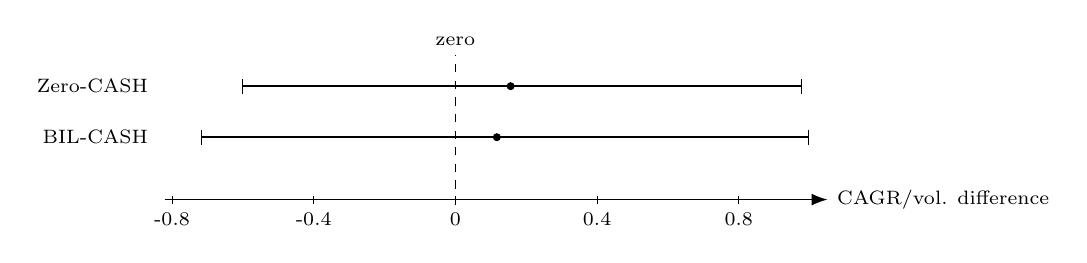
\begin{tikzpicture}[x=4.5cm,y=0.72cm]
    \draw[-{Latex[length=2mm]},line width=0.4pt] (-0.82,0) -- (1.05,0) node[right,font=\scriptsize] {CAGR/vol. difference};
    \foreach \x/\lab in {-0.8/-0.8,-0.4/-0.4,0/0,0.4/0.4,0.8/0.8} {
        \draw[line width=0.3pt] (\x,0.07) -- (\x,-0.07);
        \node[below,font=\scriptsize] at (\x,-0.07) {\lab};
    }
    \draw[dashed,line width=0.35pt] (0,-0.1) -- (0,2.55);
    \node[above,font=\scriptsize] at (0,2.55) {zero};

    \node[anchor=east,font=\scriptsize] at (-0.84,2.0) {\cashzero{}};
    \draw[line width=0.65pt] (\ZeroBootstrapLower,2.0) -- (\ZeroBootstrapUpper,2.0);
    \draw[line width=0.5pt] (\ZeroBootstrapLower,1.87) -- (\ZeroBootstrapLower,2.13);
    \draw[line width=0.5pt] (\ZeroBootstrapUpper,1.87) -- (\ZeroBootstrapUpper,2.13);
    \fill (\ZeroBootstrapMeanDelta,2.0) circle (1.45pt);

    \node[anchor=east,font=\scriptsize] at (-0.84,1.1) {\cashbil{}};
    \draw[line width=0.65pt] (\BilBootstrapLower,1.1) -- (\BilBootstrapUpper,1.1);
    \draw[line width=0.5pt] (\BilBootstrapLower,0.97) -- (\BilBootstrapLower,1.23);
    \draw[line width=0.5pt] (\BilBootstrapUpper,0.97) -- (\BilBootstrapUpper,1.23);
    \fill (\BilBootstrapMeanDelta,1.1) circle (1.45pt);
\end{tikzpicture}
\caption{Pairwise bootstrap 5th--95th percentile ranges for differences in the report-specific CAGR-to-annualized-volatility ratio. Both ranges cross zero; dots mark bootstrap mean differences. These are not 95\% confidence intervals and should not be read as the retained-set White Reality Check.}
\label{fig:bootstrap-sharpe-ci}
\end{figure}

Figure~\ref{fig:bootstrap-sharpe-ci} makes pairwise mean-path uncertainty visible. Short strategy labels are used for readability; full candidate identifiers are reported in the project outputs. The \cashzero{} values are taken unchanged from the existing V3 pairwise output and the \cashbil{} values from the existing V7 output; neither is recomputed from the expected-seed canonical Sharpe values in Table~\ref{tab:combined-ranking}.

The ranges cross zero and the WRC p-values are high. The appropriate conclusion is not that the learning approach fails, but that the aligned evidence does not justify a strong alpha or superiority claim.

\section{Robustness and Practical Feasibility}

\subsection{Is Performance Broad-Based Across Regimes?}

Regime analysis asks whether performance is broad-based or concentrated in particular market environments. The final corrected regime-winner evidence is split by cash protocol and remains mixed: TD3 case-study candidates lead in selected \cashzero{} slices, while deterministic benchmarks and momentum-style rules win many regimes, especially under \cashbil{}.

Figure~\ref{fig:regime-winners} summarizes the mixed regime evidence and reinforces the cautious interpretation. Within the post-2022 slices in which both strategy types are observed, learning candidates lead some cells but are not all-weather dominant. Regime dependence is especially important because a strategy that ranks well on average can still be practically fragile if performance is concentrated in a narrow set of historical conditions. The COVID shock/recovery and post-COVID liquidity rows predate the TD3 out-of-sample histories and contain only the 14 deterministic benchmarks; their winners are therefore benchmark-only by construction and are not evidence that TD3 lost those regimes.

\begin{figure}[H]
\centering
\scriptsize
\setlength{\tabcolsep}{3pt}
\renewcommand{\arraystretch}{1.12}
\textbf{Panel A: \cashzero{} regime winners}\\[0.35em]
\begin{adjustbox}{max width=\textwidth}
\begin{tabular}{@{}L{0.22\textwidth} C{0.15\textwidth} C{0.15\textwidth} C{0.15\textwidth} C{0.15\textwidth} C{0.15\textwidth}@{}}
\toprule
Regime & Sharpe & Max DD & Cum. return & Mandate & Composite \\
\midrule
AI / risk-on recovery & Roll. Markowitz & V8 TD3 uncapped & BuyHold BTC & V8 TD3 uncapped & Roll. Markowitz \\
Calendar 2022 & BuyHold GLD & V8 TD3 uncapped & BuyHold GLD & BuyHold GLD & BuyHold GLD \\
Calendar 2023 & V8 TD3 uncapped & V8 TD3 uncapped & BuyHold BTC & V8 TD3 uncapped & Eq. Weight risky \\
Calendar 2024 & Eq. Weight risky & V7 TD3 cap 0.80 & BuyHold BTC & V7 TD3 cap 0.80 & Roll. Markowitz \\
Calendar 2025 & BuyHold GLD & Roll. min-var & BuyHold GLD & Roll. min-var & BuyHold GLD \\
Calendar 2026 YTD & BuyHold SPY & Trend SPY/CASH & Momentum & BuyHold SPY & BuyHold SPY \\
COVID shock / recovery & BuyHold BTC & BuyHold TLT & BuyHold BTC & Risk-adj. mom. & Risk-adj. mom. \\
Inflation / hiking shock & BuyHold GLD & V8 TD3 uncapped & BuyHold GLD & BuyHold GLD & BuyHold GLD \\
Post-COVID liquidity & BuyHold SPY & 60/40 & Risk-adj. mom. & 60/40 & BuyHold SPY \\
Recent / late test window & BuyHold GLD & Trend SPY/CASH & Momentum & Roll. min-var & BuyHold GLD \\
\bottomrule
\end{tabular}
\end{adjustbox}

\vspace{0.8em}
\textbf{Panel B: \cashbil{} regime winners}\\[0.35em]
\begin{adjustbox}{max width=\textwidth}
\begin{tabular}{@{}L{0.22\textwidth} C{0.15\textwidth} C{0.15\textwidth} C{0.15\textwidth} C{0.15\textwidth} C{0.15\textwidth}@{}}
\toprule
Regime & Sharpe & Max DD & Cum. return & Mandate & Composite \\
\midrule
AI / risk-on recovery & Risk-adj. mom. & Risk-adj. mom. & BuyHold BTC & Risk-adj. mom. & Risk-adj. mom. \\
Calendar 2022 & BuyHold GLD & Risk-adj. mom. & BuyHold GLD & BuyHold GLD & BuyHold GLD \\
Calendar 2023 & Risk-adj. mom. & Risk-adj. mom. & BuyHold BTC & Risk-adj. mom. & Risk-adj. mom. \\
Calendar 2024 & Risk-adj. mom. & Risk-adj. mom. & BuyHold BTC & Risk-adj. mom. & Risk-adj. mom. \\
Calendar 2025 & Risk-adj. mom. & Risk-adj. mom. & BuyHold GLD & Risk-adj. mom. & BuyHold GLD \\
Calendar 2026 YTD & Risk-adj. mom. & Risk-adj. mom. & Momentum & Risk-adj. mom. & Risk-adj. mom. \\
COVID shock / recovery & BuyHold BTC & Risk-adj. mom. & BuyHold BTC & Risk-adj. mom. & Risk-adj. mom. \\
Inflation / hiking shock & BuyHold GLD & Risk-adj. mom. & BuyHold GLD & BuyHold GLD & BuyHold GLD \\
Post-COVID liquidity & BuyHold SPY & 60/40 & Risk-adj. mom. & 60/40 & BuyHold SPY \\
Recent / late test window & Risk-adj. mom. & Risk-adj. mom. & Momentum & Risk-adj. mom. & Risk-adj. mom. \\
\bottomrule
\end{tabular}
\end{adjustbox}

\vspace{0.35em}
\parbox{0.94\textwidth}{\footnotesize\emph{Note:} Cells report the strategy with the strongest metric within each regime in the final corrected cash-specific summaries. The COVID shock/recovery and post-COVID liquidity rows use 14 benchmark strategies only because the TD3 out-of-sample histories start on 7 January 2022; other rows use the strategies available on their dates.}
\caption{Regime winners by evaluation metric under \cashzero{} and \cashbil{}. No strategy dominates the post-2022 slices. The two pre-2022 rows are benchmark-only comparisons and cannot be used to infer TD3 performance in those regimes.}
\label{fig:regime-winners}
\end{figure}

\subsection{Do Competitive Candidates Satisfy Practical Constraints?}

Mandate analysis evaluates whether seed-aggregated strategy metrics satisfy hard practical constraints rather than only ranking by a smooth score. No strategy passes the conservative or moderate profile. Under each cash protocol, \AggressiveFeasibleCount{} deterministic benchmarks---rolling long-only Markowitz, rolling minimum variance, and 60/40 SPY/TLT---pass the aggressive profile; \TDThreeFeasibleCount{} seed-aggregated TD3 candidates pass any profile. At the individual-run level, 3 of 10 BIL V3 seeds and 1 of 10 BIL V7 seeds pass the aggressive profile, but no TD3 passes consistently across seeds. This is a feasibility diagnostic under normative test thresholds, not a universal suitability judgment.

Pareto evidence is less restrictive than hard feasibility. V3 and V4 lie on both reported frontiers under \cashzero{}. Under \cashbil{}, V3 lies on both frontiers and V8 on the full frontier only. V7 does not remain on either seed-aggregated frontier. Pareto membership is therefore supported conditionally on the chosen objectives, but it does not override failed hard filters or establish statistical superiority.

\begin{table}[htbp]
\centering
\caption{Practical feasibility interpretation.}
\label{tab:practical-feasibility}
\footnotesize
\setlength{\tabcolsep}{5pt}
\renewcommand{\arraystretch}{1.22}
\begin{tabularx}{\textwidth}{@{}L{0.22\textwidth} L{0.36\textwidth} Y@{}}
\toprule
Evaluation & Finding & Interpretation \\
\midrule
Hard mandate filters & No TD3 passes; three benchmarks pass the aggressive profile in each protocol. & Tested TD3 practical feasibility is not supported. \\
Mandate scoring & Rolling min-var leads conservative/moderate; rolling long-only Markowitz leads aggressive. & Winners are identical across cash protocols; scores remain normative diagnostics. \\
Pareto analysis & Zero-CASH has V3/V4 on both frontiers; BIL-CASH has V3 on both and V8 on the full frontier only. & Conditional tradeoff competitiveness, not universal feasibility. \\
Overall interpretation & BuyHold GLD leads the combined score, while different benchmarks pass hard filters. & Ranking leadership, feasibility, and Pareto membership remain separate claims. \\
\bottomrule
\end{tabularx}
\end{table}

\subsection{How Sensitive Are Results to Additional Execution Spreads?}

Execution-spread robustness is a reporting-only post-training proxy stress test. It does not retrain TD3 and does not create new final winners. Its purpose is to test whether selected histories are sensitive to explicit additional spread assumptions, not to estimate live execution quality.

The selected learning candidates degrade more than the simple trend/cash benchmark. Under stress spreads, \cashzero{} TD3 V3 clean macro cap 0.70 has an annualized return delta of -0.0139 and Sharpe delta of -0.1321. \cashbil{} TD3 V7 macro+GARCH cap 0.80 has an annualized return delta of -0.0128 and Sharpe delta of -0.1180. The Trend SPY/CASH benchmark has a Sharpe delta around -0.0132.

Figure~\ref{fig:execution-spread-sharpe-degradation} shows the same comparison. It is a sensitivity result for the retained V3/V7 histories, not a re-ranking of the aligned 19-strategy universes. The stress scenario uses base half-spreads of 3, 5, 5, 50, and 0 bps for SPY, TLT, GLD, BTC-USD, and CASH, respectively. These are scaled around each history's median 12-week rolling portfolio volatility with $\beta=0.5$ and applied to stored asset-level target-to-prior-target turnover. They are proxy assumptions, not observed quotes, market impact, or an account-specific cost estimate.

\begin{figure}[htbp]
\centering
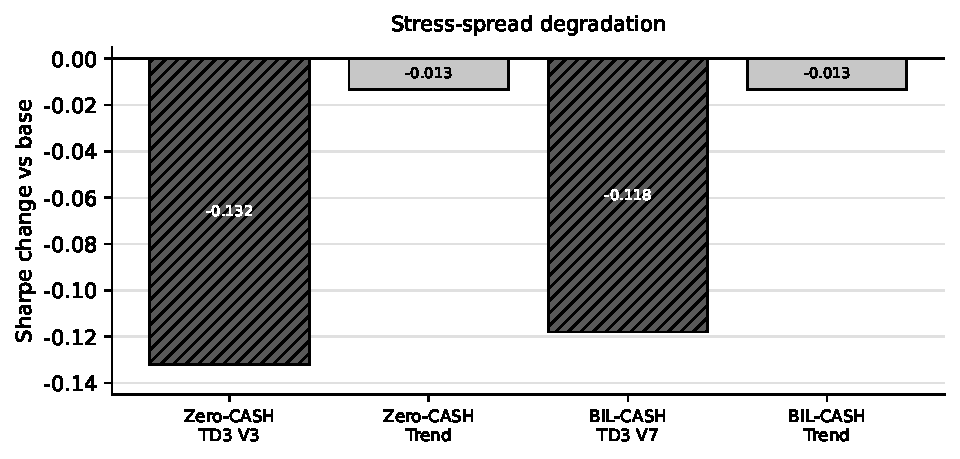
\includegraphics[width=0.82\textwidth]{execution_spread_sharpe_degradation.pdf}
\caption{Change in Sharpe ratio under a reporting-only post-training proxy-spread stress. The selected TD3 histories degrade more than Trend SPY/CASH in both cash protocols. The exercise revalues existing histories; it neither uses quote-level spreads nor retrains policies or selects new winners.}
\label{fig:execution-spread-sharpe-degradation}
\end{figure}

\subsection{Does the 60-Episode Budget Look Obviously Insufficient?}

Training-budget convergence checks whether the 60-episode protocol appears obviously undertrained. The convergence run covers 320 repeated histories: 4 candidates, 4 training budgets, 5 seeds, and 4 folds, across 30, 60, 100, and 150 episodes. These histories share the same market record and are not 320 independent market samples.

Under the pre-specified diagnostic thresholds---0.10 in Sharpe, 0.03 in absolute max drawdown, and 25\% in relative turnover versus 60 episodes---the evidence does not show that 60 episodes is materially undertrained for the selected candidate-cap pairs. Zero rows support undertraining of the 60-episode budget; three pairs have their best Sharpe at 60 episodes, while the V5 no-volatility \cashzero{} pair peaks at 30 episodes. Additional training does not improve the selected pairs and, in several cases, degrades Sharpe or increases turnover. Figure~\ref{fig:training-budget-sharpe-convergence} shows the two candidates used in the main benchmark comparison.

\begin{figure}[htbp]
\centering
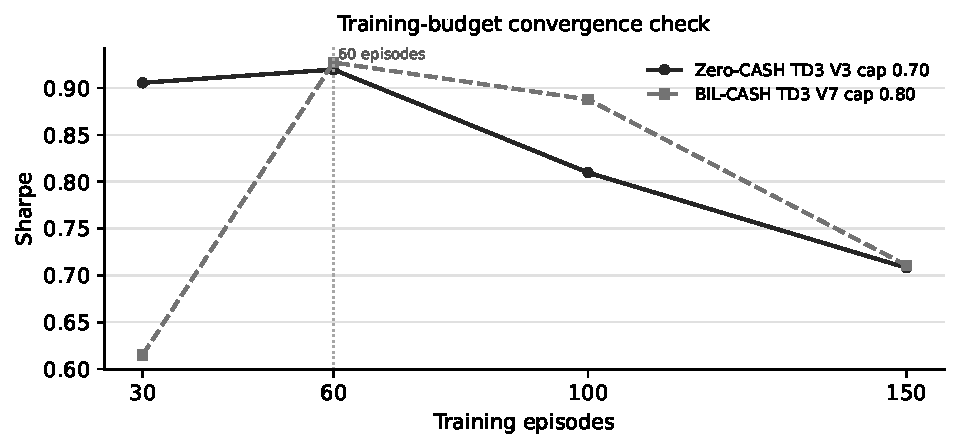
\includegraphics[width=0.82\textwidth]{training_budget_sharpe_convergence.pdf}
\caption{Training-budget Sharpe diagnostic for two main-comparison TD3 candidates, based on five seeds and four related walk-forward folds per budget. The 60-episode setting is not flagged as obviously undertrained, but the non-monotone paths do not establish global convergence or optimality.}
\label{fig:training-budget-sharpe-convergence}
\end{figure}

\section{Discussion}

\subsection{What the Evaluation Stack Reveals}

The main lesson from the experiment is not that TD3 wins or fails. The main lesson is that the interpretation of a DRL portfolio result changes materially as evaluation layers are added. Exact-window regeneration replaces the previous TD3-led ordering with BuyHold GLD leadership; computing metrics before seed aggregation then removes the artificial risk smoothing of the average-return path and moves the best TD3 canonical Sharpe to tenth in both protocols. Statistical diagnostics, hard feasibility, Pareto membership, regime dependence, spread stress, and training-budget checks answer different questions about the same case study. Ranking competitiveness, statistical credibility, practical feasibility, and the economic object being measured cannot be collapsed into one result.

Under that stack, ranking competitiveness is supported only in a limited diagnostic sense. V3 ranks fourth by mandate-aware score under \cashzero{} and V7 ranks seventh under \cashbil{}, but both rank tenth by canonical Sharpe and neither exceeds Trend SPY/CASH. The displayed pairwise mean-path ranges cross zero and retained-set WRC p-values are high. The Pareto members are different TD3 candidates and remain conditional on the objective set. None of these findings can be converted into an alpha or deployment claim.

\subsection{What the Evaluation Stack Rejects}

The boundary of the result is equally important. Mean-path bootstrap ranges include zero and White Reality Check p-values do not support statistical superiority for the retained five-candidate set. These diagnostics do not constitute inference on the expected-seed metric distribution. No seed-aggregated TD3 candidate passes a hard mandate profile. Selected case-study histories are more sensitive to additional spread assumptions than Trend SPY/CASH. The cash assumption changes both the prior within-TD3 selection and the highest-ranked seed-aggregated TD3, from V3 under \cashzero{} to V7 under \cashbil{}.

\subsection{Why Benchmarks Matter}

The benchmark set is not a collection of weak strawmen. It includes deterministic rules that capture diversification, trend following, risk-off behavior, momentum, risk parity, and classical optimization ideas. The Trend SPY/CASH benchmark remains a strong comparator in both cash protocols.

The learning approach must be compared against these strategies before any claim about dynamic allocation value is credible. A model that ranks well only against weak baselines would not be persuasive in applied finance.

\subsection{Practical Feasibility as a Separate Claim}

Practical feasibility is not implied by a favorable ranking. The mandate, Pareto, regime, execution-spread, and training-budget layers show that implementation-relevant constraints can alter the interpretation of the same return history. A candidate can remain attractive on standard metrics while still failing hard mandate filters, degrading under spread stress, or depending on a particular cash assumption.

\subsection{Methodological Contribution}

The main contribution is a falsification-oriented evaluation framework for DRL portfolio allocation. The paper shows how the interpretation of a DRL portfolio result changes when the case-study learner is evaluated through costs, cash assumptions, benchmark regeneration, statistical validation, mandate/Pareto feasibility, regime analysis, execution-spread stress, and convergence checks.

The evidence supports a bounded claim: selected TD3 candidates remain visible in the mandate-aware ranking and on tested Pareto frontiers, but no TD3 leads the combined universe, reaches the leading canonical-Sharpe positions, passes a hard mandate profile consistently, or establishes statistical superiority.

This separation is the paper's main contribution: it turns a single backtest ranking into a structured evidence hierarchy.

\begin{table}[htbp]
\centering
\caption{Claim versus evidence.}
\label{tab:claim-evidence}
\footnotesize
\setlength{\tabcolsep}{5pt}
\renewcommand{\arraystretch}{1.22}
\begin{tabularx}{\textwidth}{@{}L{0.25\textwidth} L{0.13\textwidth} Y@{}}
\toprule
Claim & Assessment & Evidence \\
\midrule
Ranking competitiveness. & Limited support & V3 ranks fourth by mandate-aware score under \cashzero{} and V7 seventh under \cashbil{}, but both rank tenth by canonical Sharpe; BuyHold GLD ranks first. \\
Statistical superiority. & Not supported & Both displayed bootstrap ranges include zero; retained-five-candidate WRC p-values do not reject the search-adjusted null. \\
Cash assumption matters. & Supported for selection & The prior TD3 selection changes from V5 to V8, and the highest-ranked seed-aggregated TD3 changes from V3 under \cashzero{} to V7 under \cashbil{}. \\
60 episodes is undertrained. & No evidence & Longer budgets do not materially improve the selected pairs and can increase turnover or reduce Sharpe. \\
Execution assumptions matter. & Supported & Stress spreads degrade selected learning candidates more than Trend SPY/CASH. \\
Hard TD3 feasibility. & Not supported & No TD3 passes any tested profile; three deterministic benchmarks pass the aggressive profile in each protocol. \\
Pareto competitiveness. & Conditional support & V3/V4 enter both \cashzero{} frontiers; under \cashbil{}, V3 enters both and V8 the full frontier only, conditional on the declared objectives. \\
Custom scores are sufficient. & Not supported & Scores are diagnostic; standard metrics and statistical validation remain necessary. \\
Benchmarks are weak. & Not supported & Regenerated deterministic benchmarks remain strong comparators across metrics and regimes. \\
\bottomrule
\end{tabularx}
\end{table}

\section{Limitations}

The compact universe makes allocations interpretable but limits external validity. It is mainly U.S.-centric, omits credit, real estate, international equities, and broad commodities beyond gold, and uses one idiosyncratic crypto asset. Synthetic CASH and BIL are alternative liquidity approximations, not interchangeable definitions of a risk-free asset or a complete representation of operational cash.

The study observes one market history. Expanding walk-forward folds and multiple random seeds test temporal and training variation, but the folds remain related and repeated TD3 histories are not independent market samples. TD3 is also the only DRL learner examined. The findings therefore evaluate this framework through one algorithmic case study; they do not establish that the same ranking or sensitivity patterns hold for other learners, reward designs, or historical samples.

Candidate flexibility and benchmark flexibility are not identical. The TD3 layer searches feature families, caps, seeds, and folds, whereas the deterministic rules use pre-specified constructions. White Reality Check covers five retained candidate-cap policies per cash protocol, not all 20 feature-cap configurations in the final grid. Its conclusion also depends on the benchmark comparator, return differential, and resampling design, and cannot correct for every earlier research choice. Similarly, mandate thresholds are normative stress tests rather than universal investor requirements, and Pareto membership depends on the selected objectives.

Exact date alignment removes the previous horizon mismatch but does not create independent market observations. For each candidate, four folds are concatenated within seed and nonlinear metrics are computed separately on ten complete OOS histories before their arithmetic mean is taken. This estimates expected performance over training seeds, not the result of one deployable policy. The synthetic date-wise average path reduces individual-policy volatility by roughly 18--34\% across the selected candidates and is therefore retained only as a diversification diagnostic. Its net returns, turnover, and costs are averages of quantities already computed in separate policies; they are not recomputed from netted ensemble weights. Deterministic benchmarks have no training-seed distribution. Their missing seed dispersion is treated as unavailable and neutral rather than zero in the stability component, but the robust and mandate-aware scores remain diagnostic rather than a primary TD3-versus-benchmark claim. Benchmark signals, weights, and costs are retained from their causal full histories and filtered to the common window; their first aligned row preserves pre-window benchmark position state.

The pairwise bootstrap report uses both a different economic object and a different risk-adjusted-return estimator from the combined ranking: the synthetic mean path and CAGR divided by annualized volatility, rather than the mean across per-seed canonical Sharpe values. Its ranges remain internally pairwise and unchanged, but their numerical summaries cannot be reconciled directly with Table~\ref{tab:combined-ranking}. White Reality Check is separate again: it resamples centered weekly return differentials and does not use either ratio. A hierarchical inference procedure that jointly preserves seed and serial dependence has not been implemented.

Execution remains approximate. Asset-specific transaction costs and the spread stress make turnover economically visible, but they omit market impact, order-book depth, latency, capacity, routing, taxes, custody, and live-forward execution. The training-budget analysis is only a diagnostic against obvious undertraining over four tested budgets; non-monotone Sharpe paths do not prove global convergence. These limits restrict deployment and generalization claims without negating the value of the evaluation hierarchy.

\section{Conclusion}

This paper asks whether a falsification-oriented framework can separate claims that a conventional backtest often conflates. On an exact \AlignedWeeks{}-date comparison with metrics computed before seed aggregation, BuyHold GLD leads both combined rankings. V3 is the best TD3 by mandate-aware score under \cashzero{} at rank four and V7 under \cashbil{} at rank seven; both rank tenth by canonical Sharpe. Pairwise mean-path ranges cross zero and White Reality Check does not support superiority for the retained five-candidate set. No seed-aggregated TD3 passes a tested hard mandate profile. V3/V4 enter both \cashzero{} Pareto frontiers; under \cashbil{}, V3 enters both and V8 the full frontier only.

The strongest defensible conclusion is therefore methodological. Current evidence supports only bounded diagnostic ranking and Pareto claims; it does not support statistical superiority or consistent hard TD3 feasibility under the tested rules. The paper's contribution is the evaluation protocol, exact-date and seed-level reproducibility layer, and disciplined boundary around claims, not a new TD3 method or a deployable return advantage.

\bibliographystyle{plainnat}
\bibliography{references}

\clearpage
\appendix

\section{Protocol and Reproducibility Detail}
\label{app:protocol-detail}

Table~\ref{tab:walk-forward-folds} records the expanding-window design. Feature alignment can move the first usable training row beyond the nominal start; validation and test boundaries remain fixed.

\begin{table}[htbp]
\centering
\caption{Corrected walk-forward folds.}
\label{tab:walk-forward-folds}
\footnotesize
\begin{tabularx}{\textwidth}{@{}L{0.08\textwidth} L{0.26\textwidth} L{0.24\textwidth} Y@{}}
\toprule
Fold & Training window & Validation window & Out-of-sample test window \\
\midrule
F1 & 3 Apr. 2015--25 Dec. 2020 & 1 Jan.--31 Dec. 2021 & 7 Jan.--30 Dec. 2022 \\
F2 & 3 Apr. 2015--31 Dec. 2021 & 7 Jan.--30 Dec. 2022 & 6 Jan.--29 Dec. 2023 \\
F3 & 3 Apr. 2015--30 Dec. 2022 & 6 Jan.--29 Dec. 2023 & 5 Jan.--27 Dec. 2024 \\
F4 & 3 Apr. 2015--29 Dec. 2023 & 5 Jan.--27 Dec. 2024 & 3 Jan. 2025--15 May 2026 \\
\bottomrule
\end{tabularx}
\end{table}

The corrected grid crosses V3, V4, V5, V7, and V8 with the uncapped, 0.50, 0.70, and 0.80 cap settings, seeds 7, 21, 42, 84, 101, 123, 202, 303, 404, and 505, and four folds. Its 800 histories per cash protocol share one market record and are not independent observations. Actions are projected to the capped long-only simplex before execution and replay storage; metrics use net returns after asset-specific costs. Test histories initialize at equal weights and a portfolio value of 100,000.

The fourteen comparators are buy-and-hold SPY, TLT, GLD, and BTC-USD; equal weight with and without CASH; 60/40 SPY/TLT; defensive risk-off; momentum; risk-adjusted momentum; rolling long-only Markowitz; rolling minimum variance; inverse-volatility risk parity; and Trend SPY/CASH. Their original causal histories retain any permitted pre-window indicator warm-up and position state. Comparison rows are selected by exact intersection with the TD3 index, never by taking the last 228 rows. Every aligned output contains \AlignedWeeks{} observations from \AlignedStartDate{} to \AlignedEndDate{}, with zero duplicate dates and zero missing returns.

Candidate identifiers serve different pre-specified reporting roles. The prior within-TD3 diagnostic selection uses V5 cap 0.50 under \cashzero{} and V8 cap 0.70 under \cashbil{}. Under metrics-then-average, the best combined-ranking TD3 by mandate-aware score is V3 cap 0.70 under \cashzero{} and V7 cap 0.80 under \cashbil{}; Table~\ref{tab:stat-validation} displays their already-existing Trend pairwise rows without rerunning the bootstrap. The best WRC mean-return differential remains V7 cap 0.80 in both protocols because WRC uses the synthetic mean-return differential matrix rather than the seed-aggregated ranking. The retained WRC universes are {V3 0.70, V7 0.80, V4 0.70, V8 uncapped, V5 0.50} for \cashzero{} and {V7 0.80, V3 0.70, V8 0.70, V4 0.80, V5 0.70} for \cashbil{}. These roles are defined by different estimands and are not retrospective seed selection.

\subsection{Statistical and Practical Decision Rules}

For the pairwise bootstrap, TD3 returns are averaged by date, aligned with the benchmark over \AlignedWeeks{} weeks, and resampled jointly using 1,000 replications and 12-week blocks. The reported range is the 5th--95th percentile difference in the \emph{CAGR-to-annualized-volatility ratio}; it is not a 95\% confidence interval, a canonical Sharpe interval, or expected-seed inference. White Reality Check applies 2,000 centered block-bootstrap replications with 8-week blocks to the weekly candidate-minus-benchmark net-return matrix. Its statistic is $\sqrt{T}$ times the largest candidate mean return differential; it does not use the CAGR-to-volatility ratio. Its null concerns the retained five-policy TD3 set, not the full 20-configuration grid. A high p-value fails to reject that null; the result is candidate-set dependent and is not an SPA test.

The reporting-only robust score retains its fixed weighted composite of DSR (0.30), cross-sectionally normalized Sortino (0.20), Calmar (0.20), max drawdown (0.15), stability (0.10), and discipline (0.05). Stability combines inverse normalized Sharpe dispersion (0.70) and normalized worst drawdown (0.30); discipline combines cash, turnover, and diversification diagnostics with weights 0.50, 0.30, and 0.20. TD3 seed dispersion and worst-seed drawdown are observed across ten full \AlignedWeeks{}-date histories. A deterministic benchmark has no comparable training-seed distribution, so its dispersion is missing and receives the neutral normalization value rather than an automatic zero-dispersion bonus. DSR uses the median of ten TD3 seed values and the single aligned benchmark history. The mandate-aware score retains its original drawdown multiplier and zero below $d=-0.30$. These scores remain diagnostics; canonical metrics are the primary cross-type comparison.

Hard feasibility is separate from diagnostic scores. Table~\ref{tab:mandate-thresholds} gives normative test profiles, not universal suitability standards. Experimental max-weight caps are not mandate thresholds.

\begin{table}[H]
\centering
\caption{Hard mandate thresholds used for feasibility diagnostics.}
\label{tab:mandate-thresholds}
\footnotesize
\begin{tabular}{@{}lcccc@{}}
\toprule
Profile & \makecell{Max\\drawdown} & \makecell{Max ann.\\volatility} & \makecell{Min effective\\assets} & \makecell{Max average\\turnover} \\
\midrule
Conservative & -0.10 & 0.10 & 3.00 & 0.05 \\
Moderate & -0.15 & 0.15 & 2.30 & 0.10 \\
Aggressive & -0.25 & 0.25 & 1.50 & 0.20 \\
\bottomrule
\end{tabular}
\end{table}

Execution-spread stress only revalues selected histories after training. The clean, conservative, and stress scenario base half-spreads for {SPY, TLT, GLD, BTC-USD, CASH} are {0.25, 0.50, 0.50, 3, 0}, {1, 2, 2, 15, 0}, and {3, 5, 5, 50, 0} bps. For each history, a 12-week rolling portfolio-volatility proxy scales these bases around its median with $\beta=0.5$; spread cost is the product of the resulting asset half-spread and stored asset-level target-to-prior-target turnover. This is a quote-free sensitivity proxy and excludes market impact.

The budget diagnostic compares 30, 60, 100, and 150 episodes for four candidate/cash cases, seeds 7, 21, 42, 84, and 101, and four related folds (320 histories). Materiality thresholds are 0.10 Sharpe, 0.03 absolute max drawdown, and 25\% relative turnover versus 60 episodes. It tests for obvious undertraining at 60 episodes, not a globally optimal budget or 320 independent replications.

The primary reproducibility package is stored in \texttt{outputs/paper\_seed\_aggregated\_comparison/}. It includes all 100 complete TD3 seed histories, per-seed metrics, cross-seed summaries, synthetic mean/median-path diagnostics, diversification and cost audits, seed-aggregated rankings, hard filters, mandate profiles, Pareto tables, named statistical formulas, source SHA-256 hashes, and executable validation. The earlier \texttt{outputs/paper\_aligned\_comparison/} package remains preserved as the validated date-alignment prerequisite and average-path audit record.

\end{document}
